\section{Storia} % (fold)
	\label{sec:storia}
	
	\begin{frame}[t]\frametitle{Storia}
		\begin{itemize}
			\item 1897 $\longrightarrow$ \href{http://www.wired.it/scienza/energia/2014/04/30/la-scoperta-dellelettrone/}{Scoperta dell'elettrone} da parte di Thompson 
			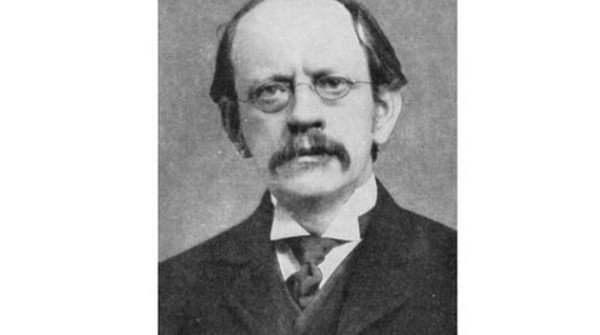
\includegraphics[width=4cm]{./img/thompson.jpg}
			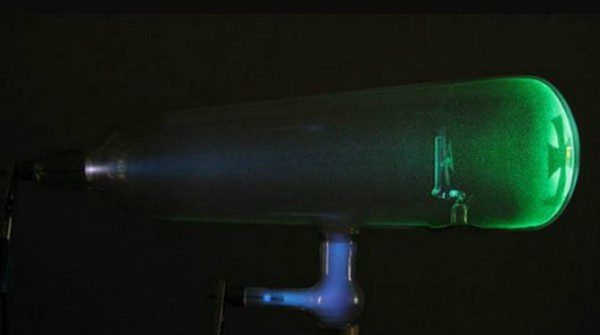
\includegraphics[width=4cm]{./img/tubo.jpg}
			\pause
			\item 1900  $\longrightarrow$ Primo modello di metallo proposto da Paul Drude (1863 – 1906) con l'atomo a panettone
			%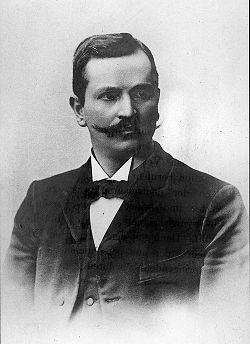
\includegraphics[width=2cm]{./img/Drude.jpg}
			\pause
			\item 1911  $\longrightarrow$ Atomo di Ernest Rutherford ( 1871 – 1937)
		\end{itemize}
	\end{frame}
	\note{2 parole sul modello a panettone e su come si sono accorti che questo non funzionava grazie allo scattering di particelle alfa elio \href{http://www.dmf.unicatt.it/~sangalet/PLS/Buone_pratiche/Esperimento_Rutherford.pdf}{fonte} 1/8000 falliva la previsione, figata che è la scienza, il modello di drude è quanto andremo noi a vedere anche se precisiamo già da ora che è falso ma rende molto bene l'idea.}

	\begin{frame}[c]\frametitle{Atomo di Rutherford}
	    
		\centering 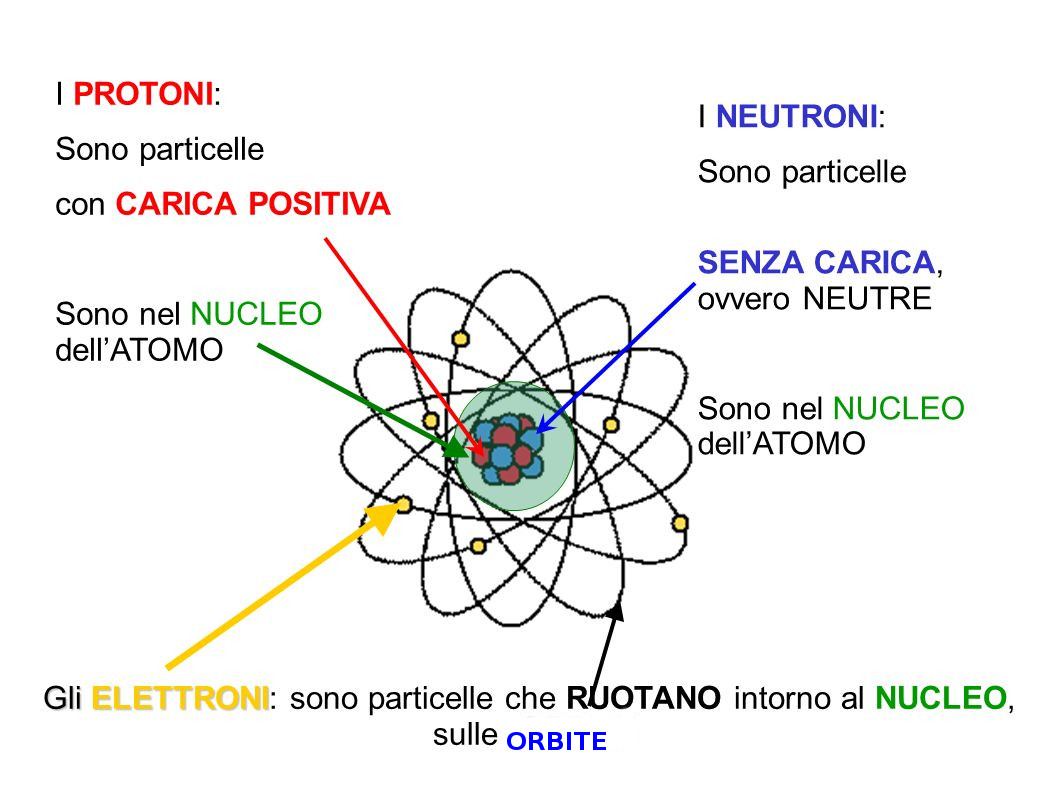
\includegraphics[width=9cm]{./img/atomo.jpg}

	\end{frame}
	\note{elettroni legati!!!!}

	\begin{frame}[c]\frametitle{Atomo di rame}
	    \begin{columns}
			\begin{column}{0.4\textwidth}
				\centering 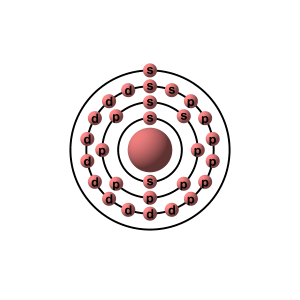
\includegraphics[width=5cm]{./img/rame.png}
			\end{column}
			\begin{column}{0.4\textwidth}
				\begin{itemize}
					\item Nucleo
					\begin{itemize}
						\item Neutroni
						\item Protoni
					\end{itemize}
					\item Elettroni
				\end{itemize}

				\vspace{0.5cm}
				
				$\longrightarrow$ Elettroni e ione!!

			\end{column}
		\end{columns}
	
	\end{frame}

	% section storia (end)

	\section{Il modello} % (fold)
	\label{sec:il_modello}
		\begin{frame}[c]\frametitle{Il metallo}
		    
		Cosa accade quando avviciniamo molti atomi?
		\centering 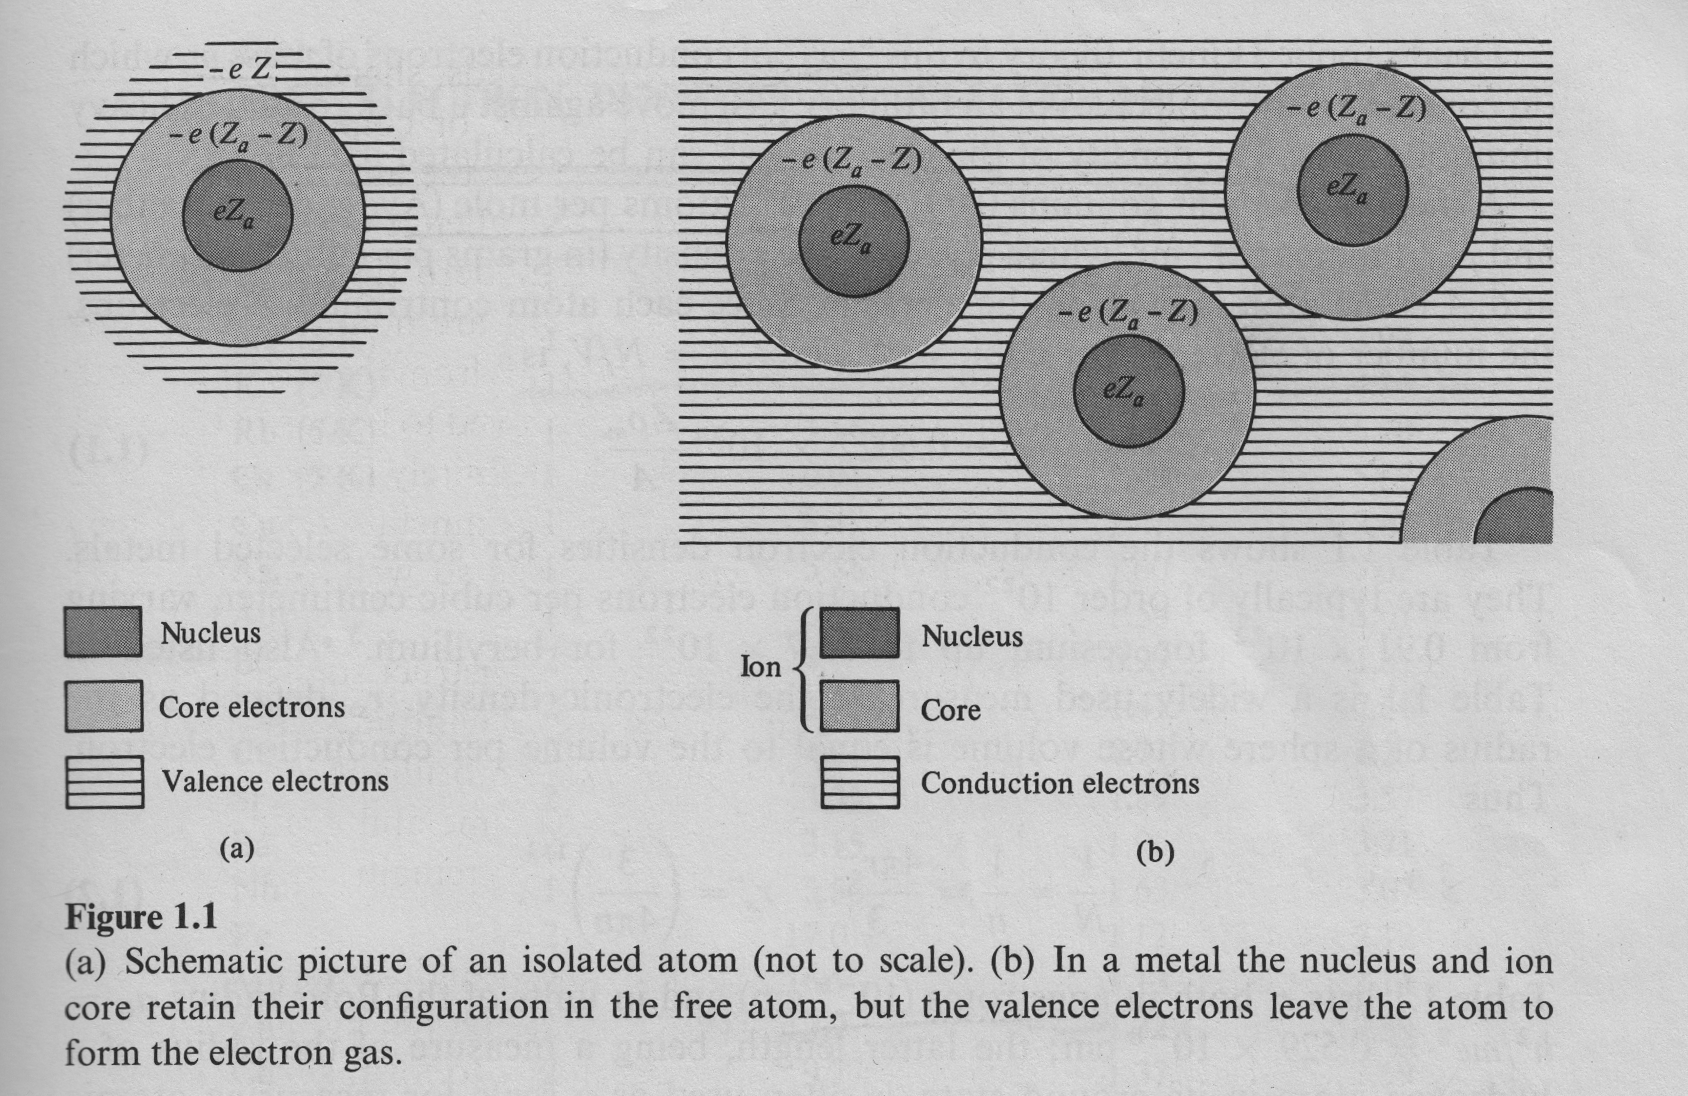
\includegraphics[width=9cm]{./img/model.png}
		
		\end{frame}

		\note{gli elettoni si muovono a caso ma la velocità media è nulla, non interagiscono fra di loro, interagiscono solo con gli atomi}
		
		\begin{frame}[c]\frametitle{Se applichiamo una differenza di potenziale?}
			\begin{columns}
				\begin{column}{0.4\textwidth}
					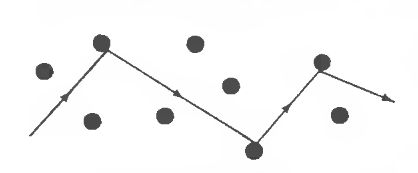
\includegraphics[width=4cm]{./img/path.png}
				\end{column}
				\begin{column}{0.7\textwidth}

					$\longrightarrow$ $V(x)$ Potenziale\\
					$\longrightarrow$ $E(x)$ Campo Elettrico
					\[
					 E (x) = - \frac{V(x1)-V(x2)}{\Delta x}
					\]
					\[
					 F \left(x\right) = q \left(x\right) E(x)
					\]

				\end{column}
			\end{columns}
			--note a mano--
		\end{frame}
		\note{gli elettroni cominciano a muoversi con una direzione preferenziale }

		\begin{frame}[c]\frametitle{Disclaimer}
		    
		\begin{center}
			\color{red}\textbf{Attenzione!!}
		\end{center}
		Questo modello funziona (ovvero fa buone previsioni) su alcuni conduttori e in condizioni normali ma è FALSO, la resistenza NON è data dagli urti degli atomi con i nuclei ma fenomeni ben più complicati che richiedono conoscenze di M.Q. e di matematica non banali per essere descritti e che pertanto non andiamo ad affrontare. Abbiamo scelto questo modello perché ci è sembrato, dal punto di vista didattico il miglior modo per introdurre l'argomento.		
		\end{frame}
	% section il_modello (end)

	\section{La corrente} % (fold)
	\label{sec:la_corrente}
	
	% section la_corrente (end)

	\section{La resistenza} % (fold)
	\label{sec:la_resistenza}
		\begin{frame}[c]\frametitle{Resistenza:Come si misura e come si calcola?}
		    Ma tutto quello che abbiamo visto come si porta alla quotidianità?			
		\end{frame}
		\begin{frame}[c]\frametitle{Resistenza:Come si misura e come si calcola?}
		    \begin{columns}
		    	\begin{column}{0.5\textwidth}
		    		\[
		    		 R = \frac{\rho L}{A}
		    		\]
		    		Dove $\rho$ è in $\Omega$ per metro\\
		    		Osservazione, l'oro non conduce poi così bene, perché allora si comprano i contatti placcati in oro?		    		
		    	\end{column}
		    	\begin{column}{0.7\textwidth}
		    		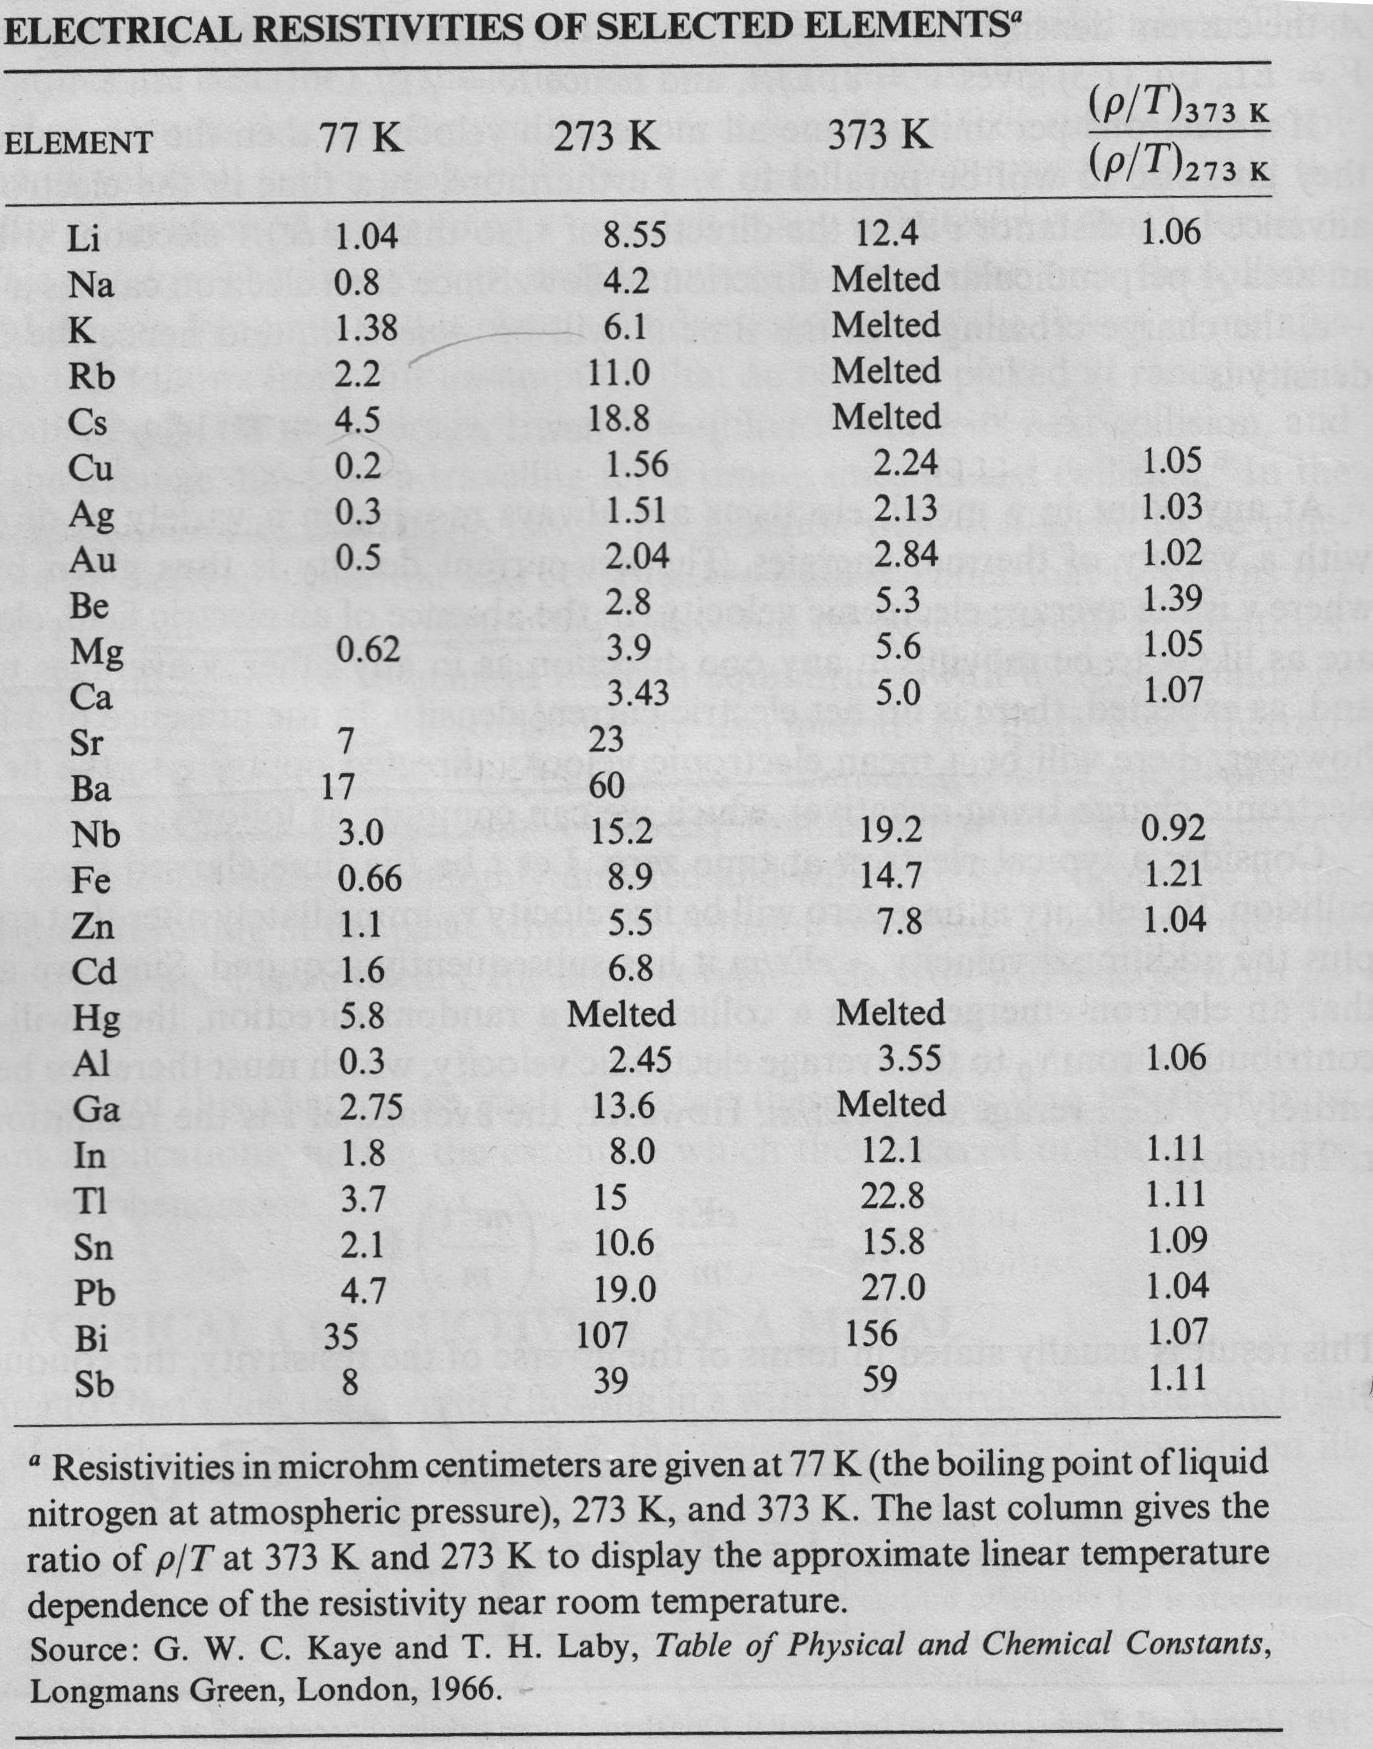
\includegraphics[width=5.5cm]{./img/rho.jpg}
		    	\end{column}
		    \end{columns}	
		\end{frame}
		\note{NON SI OSSIDANO}

		\begin{frame}[c]\frametitle{Resistori: come si comprano?}
		    \centering
		\begin{tabular}{c|c|c}
		Serie & Precisione & stato \\
		\hline
		E6	& 20\% & ormai rarissima  \\
		E12	& 10 \% & la più comune  \\
		E24	& 5  \% \\
		E48	& 2  \% & usata in rare applicazioni \\
		\end{tabular}
		
		\bigskip
		
		Nota: vengono vendute a pacchi da mille circa per 3-4 euro
		
		\end{frame}

		\begin{frame}[c]\frametitle{Resistori: come si comprano?}

		\centering La serie E 12 in tutto il suo splendore, ma perché 12?
		    
		\begin{tabular}{c|c|c|c|c|c|c|c}
			1.0 & 10 & 100 & 1.0K & 10K & 100K & 1.0M & 10M \\
			1.2 & 12 & 120 & 1.2K & 12K & 120K & 1.2M & 12M \\ 
			1.5 & 15 & 150 & 1.5K & 15K & 150K & 1.5M & 15M  \\
			1.8 & 18 & 180 & 1.8K & 18K & 180K & 1.8M & 18M  \\
			2.2 & 22 & 220 & 2.2K & 22K & 220K & 2.2M & 22M  \\
			2.7 & 27 & 270 & 2.7K & 27K & 270K & 2.7M & \\
			3.3 & 33 & 330 & 3.3K & 33K & 330K & 3.3M & \\
			3.9 & 39 & 390 & 3.9K & 39K & 390K & 3.9M & \\
			4.7 & 47 & 470 & 4.7K & 47K & 470K & 4.7M & \\
			5.6 & 56 & 560 & 5.6K & 56K & 560K & 5.6M & \\
			6.8 & 68 & 680 & 6.8K & 68K & 680K & 6.8M & \\
			8.2 & 82 & 820 & 8.2K & 82K & 820K & 8.2M & \\
		\end{tabular}
		
		\end{frame}

		\begin{frame}[c]\frametitle{Resistori: come si comprano?}
		    \centering
		E se non è in nessun elenco? lo scopriamo dopo :)\\
		Piuttosto: Come le distinguiamo?\\
		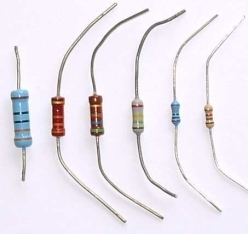
\includegraphics[width=4cm]{./img/resistenze.jpg}
		
		\end{frame}

		\begin{frame}[c]\frametitle{Resistori: come distinguono?}
			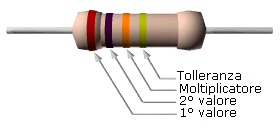
\includegraphics[width= 5cm]{./img/r5.png}
		    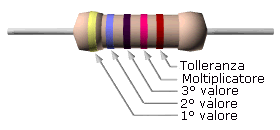
\includegraphics[width= 5cm]{./img/r1.png}\\
		    \centering 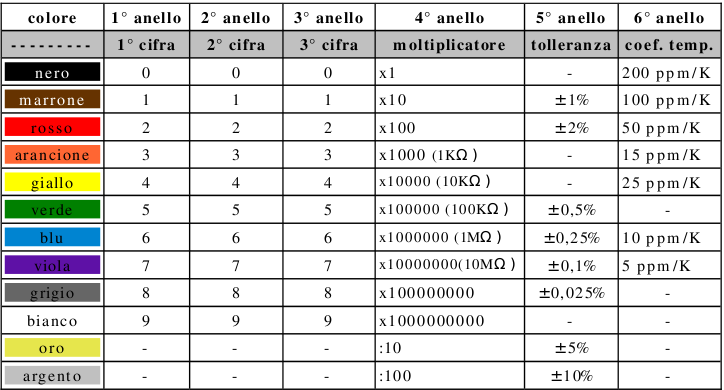
\includegraphics[width= 8cm]{./img/codice.png}
		\end{frame}
		
		\begin{frame}[c]\frametitle{Codice dei colori, un paio di esempi}
		    \centering
			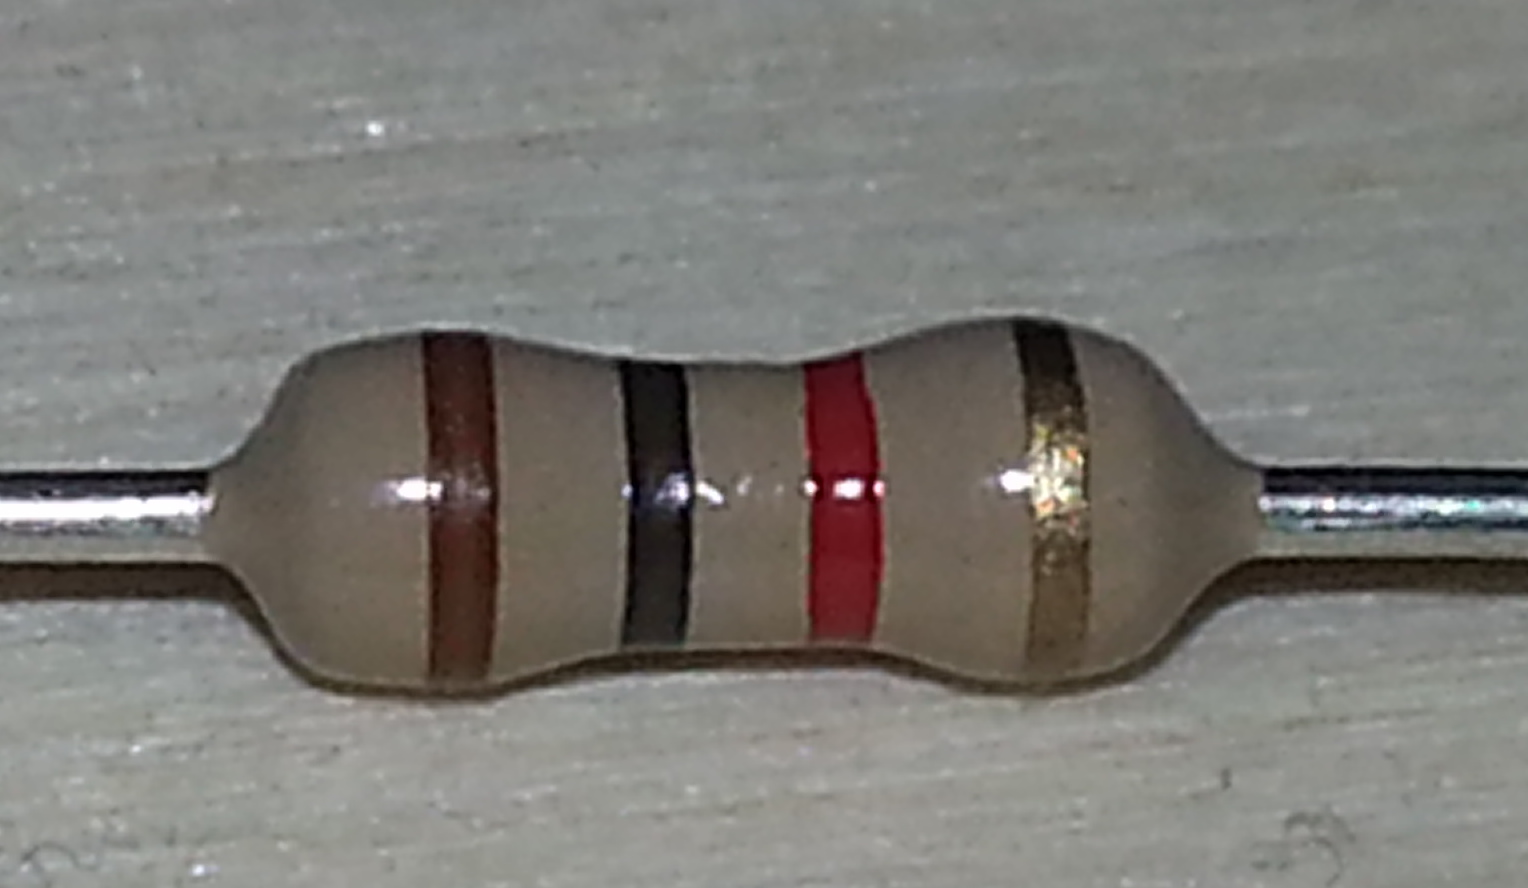
\includegraphics[width= 5 cm] {./img/E12.jpg}
			\pause
			\[
			R = 1 ~~ 0 ~~ 10^{2} \pm 5\% \Omega
			\]
		\end{frame}

		\begin{frame}[c]\frametitle{Codice dei colori, un paio di esempi}
		    \centering
			\begin{figure}[tb]
				\centering
				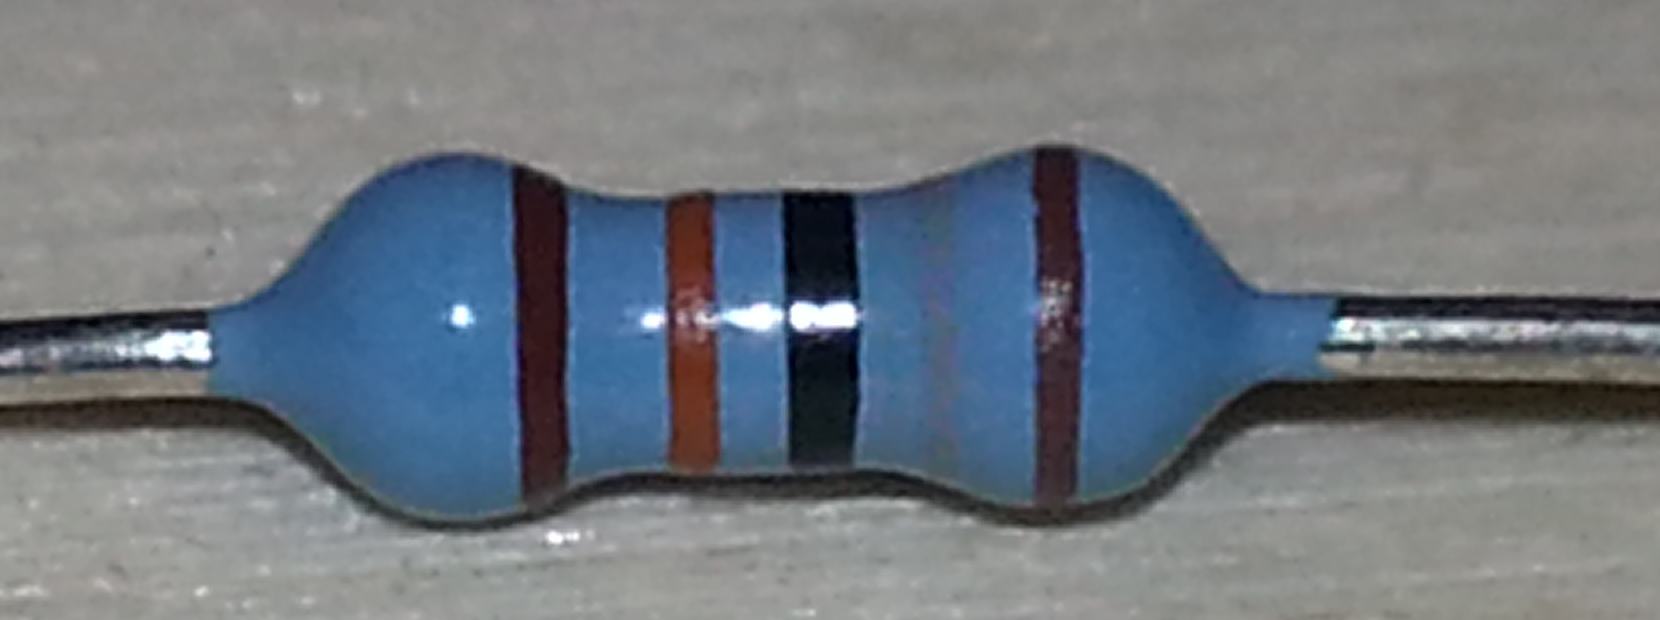
\includegraphics[width= 5 cm] {./img/E19.jpg}				
				\label{fig:figure1}
			\end{figure}

			\pause
			
			\[
			R = 1 ~~ 3 ~~ 0 ~~ 10^{8} \pm 1\% \Omega
			\]
		\end{frame}
	% section la_resistenza (end)

	\section{La differenza di potenziale} % (fold)
	\label{sec:la_differenza_di_potenziale}
		
		\begin{frame}[c]\frametitle{DDP}
		    
			Parliamo ora della differenza di potenziale
		
		\end{frame}

		\begin{frame}[c]\frametitle{DDP: un analogia molto chiarificatrice}
		    
			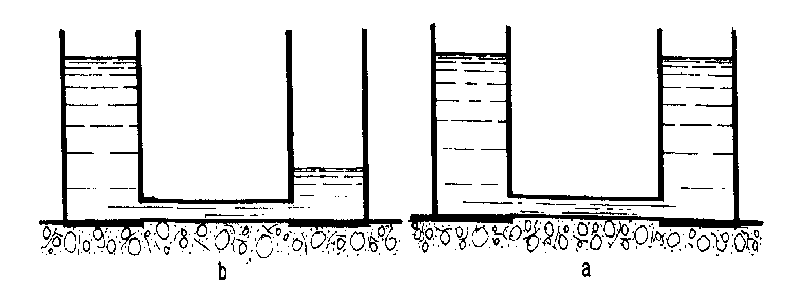
\includegraphics[width=10cm]{./img/ddp1.png}
		
		\end{frame}

		\begin{frame}[c]\frametitle{DDP: un analogia molto chiarificatrice}
		    
			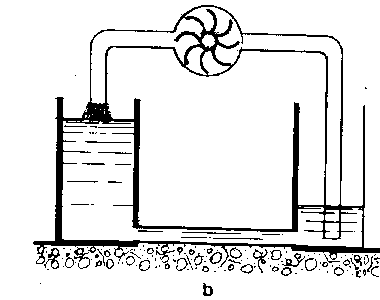
\includegraphics[width=8CM]{./img/ddp2.png}\\

			\href{http://web.mclink.it/MK1411/Apprendistato/ImpiantiElettrici/Lezioni\%20di\%20Elettrotecnica/Lezione\%201_30_Web.htm}{Fonte}
		
		\end{frame}

		\begin{frame}[c]\frametitle{Il nostro alimentatore}
		    
			\begin{figure}[h]
				\centering
				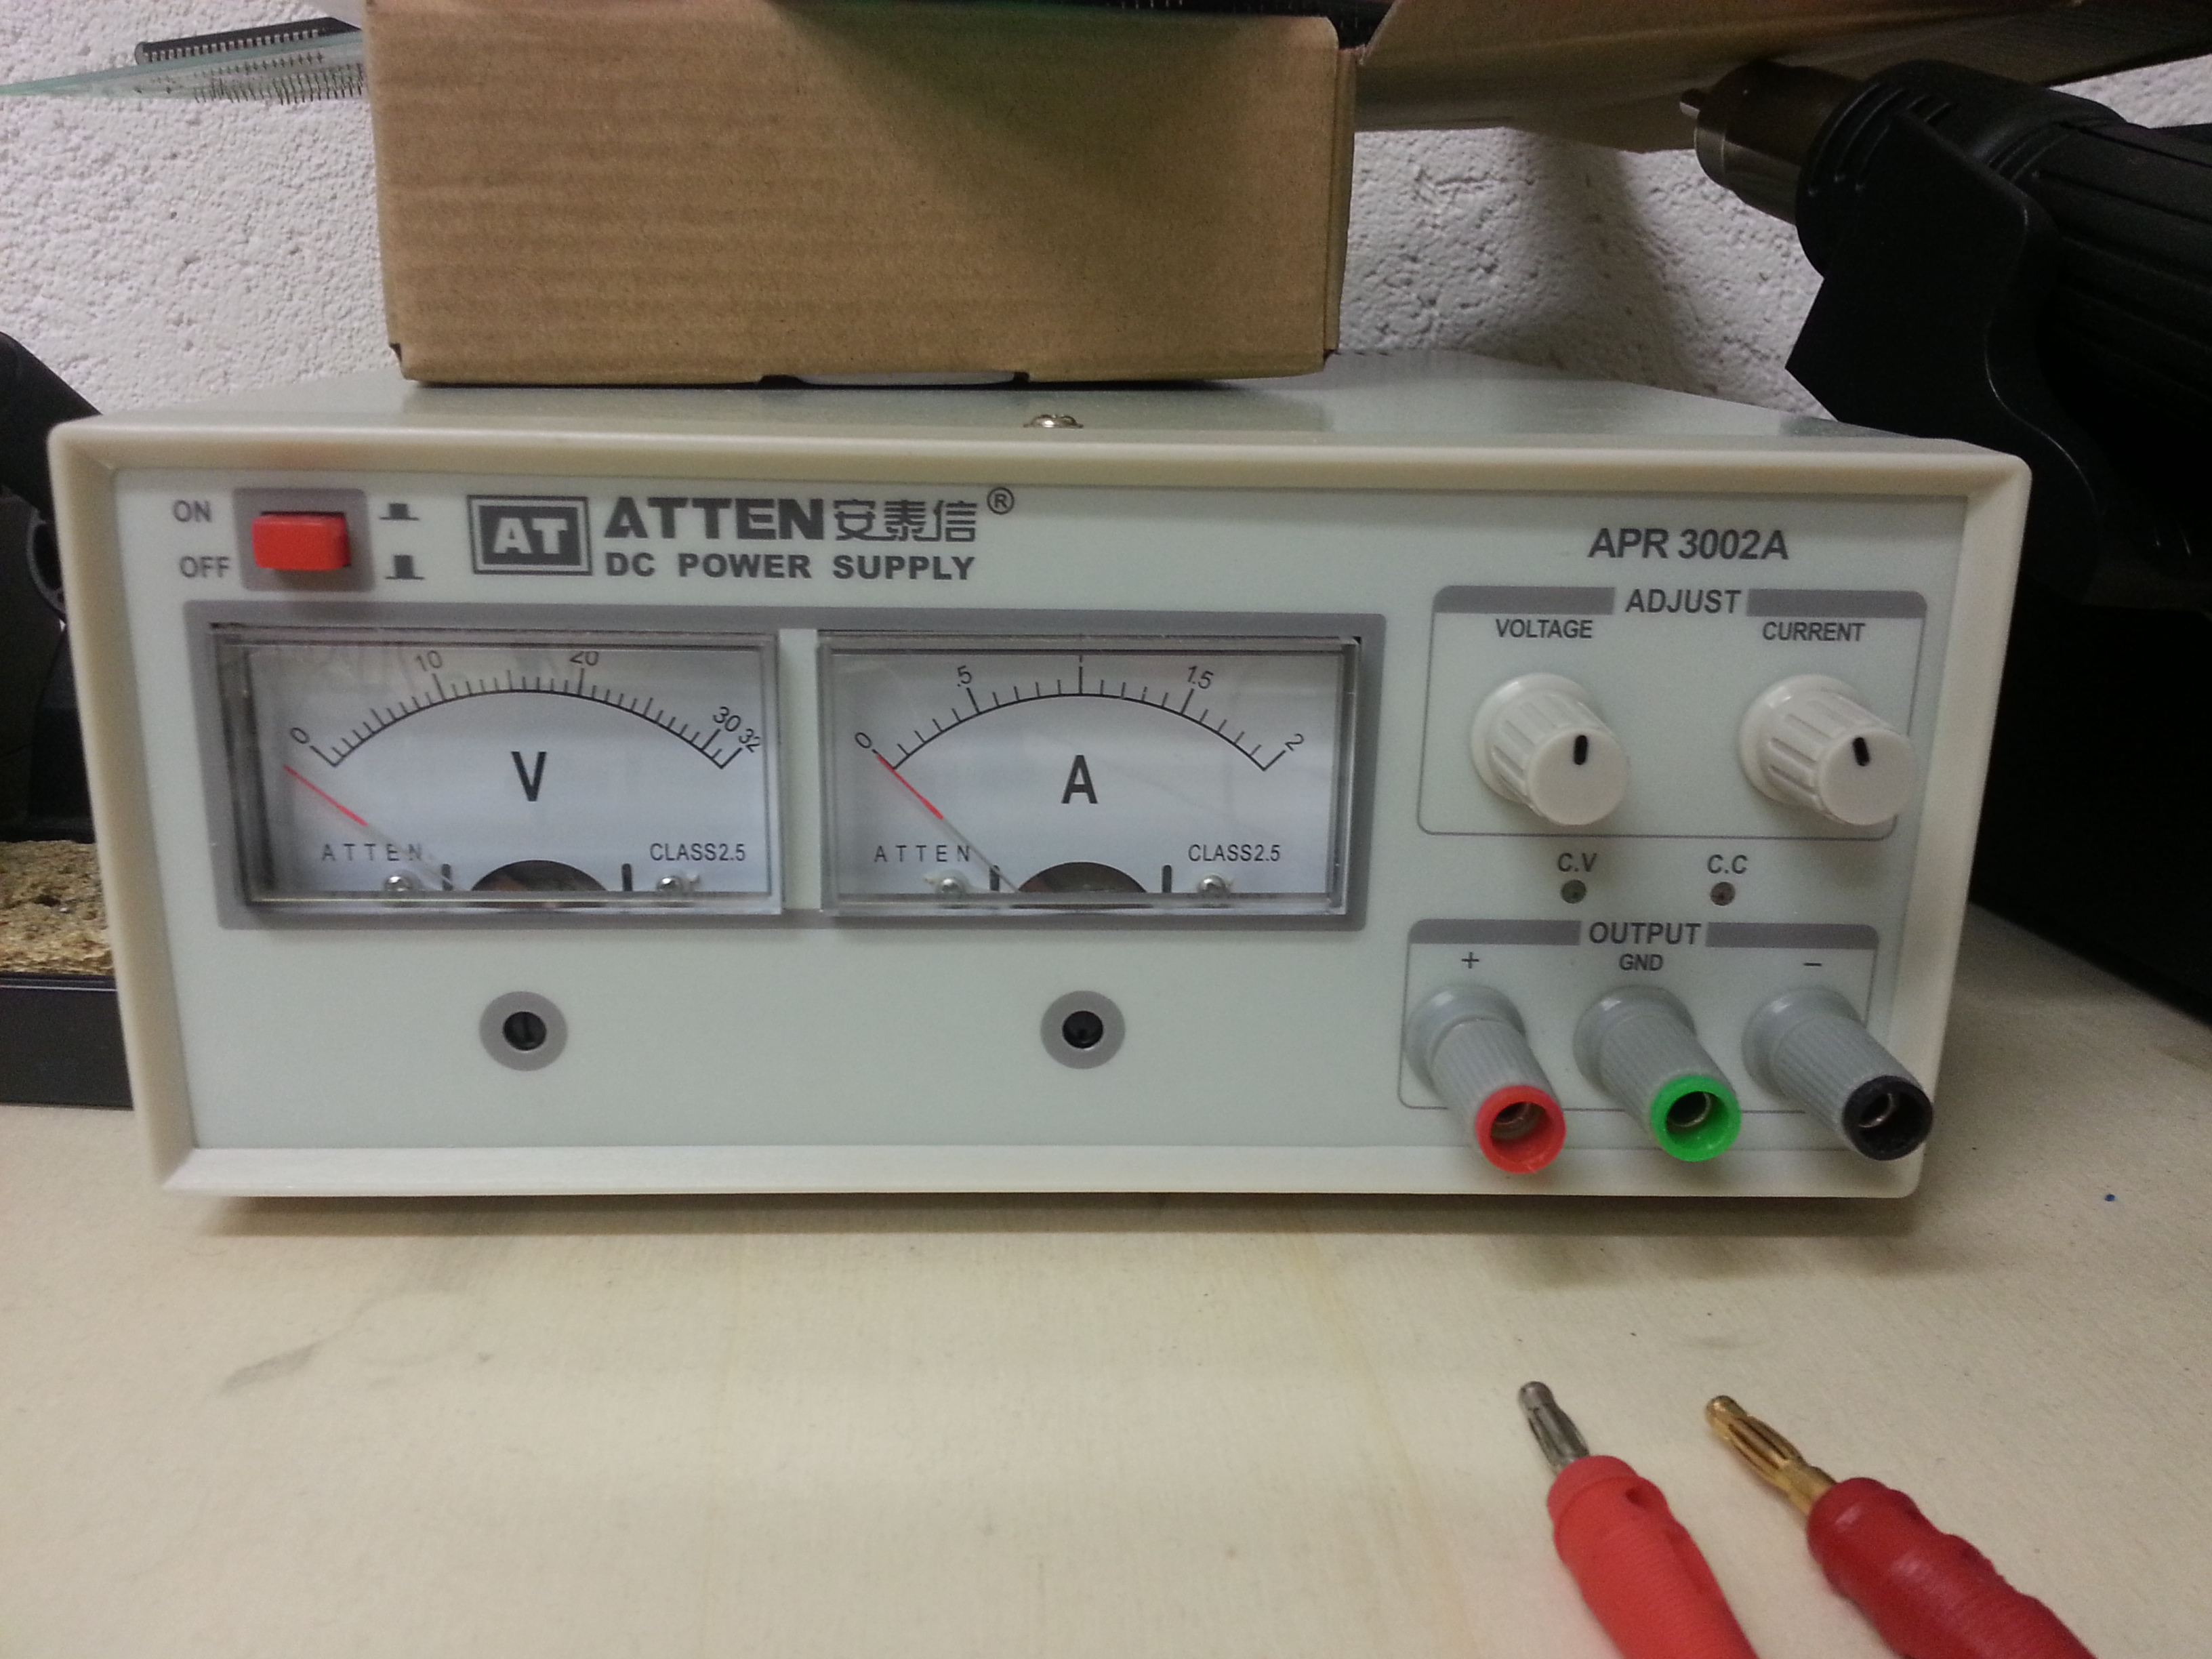
\includegraphics[width= 6cm]{./img/alim.jpg}
				\label{fig:figure2}
			\end{figure}
			\color{red}Attenzione:
			\color{black}per prima cosa azzerare le manopole e fissare il massimo della corrente.
		
		\end{frame}

	% section la_differenza_di_potenziale (end)

	\section{La legge di OHM} % (fold)
	\label{sec:la_legge_di_ohm}
		\begin{frame}[c]\frametitle{La legge di Ohm}
		     \begin{block}{Legge di Ohm}
		     	La legge di Ohm esprime la legge costitutiva di proporzionalità diretta tra la differenza di potenziale elettrico applicata ai capi di un conduttore e l'intensità della corrente elettrica che lo attraversa. 	
		     \end{block}
			\[
				V = R \times I
			\]

			\begin{itemize}
				\item Dove $V$ è la tensione $R$ è la resistenza e $I$ è la corrente.
				\pause
			 	\item \`E una relazione lineare
			 	\item Noi non l'abbiamo dimostrata e la caliamo dal celo ma la nostra prima esperienza consisterà in una sua verifica.
			 \end{itemize} 

		\end{frame}
	% section la_legge_di_ohm (end)

	\section{Il multimetro} % (fold)
	\label{sec:il_multimetro}
		\begin{frame}[c]\frametitle{I nostri multimetri}
		    
			\begin{figure}[tb]
				\centering
				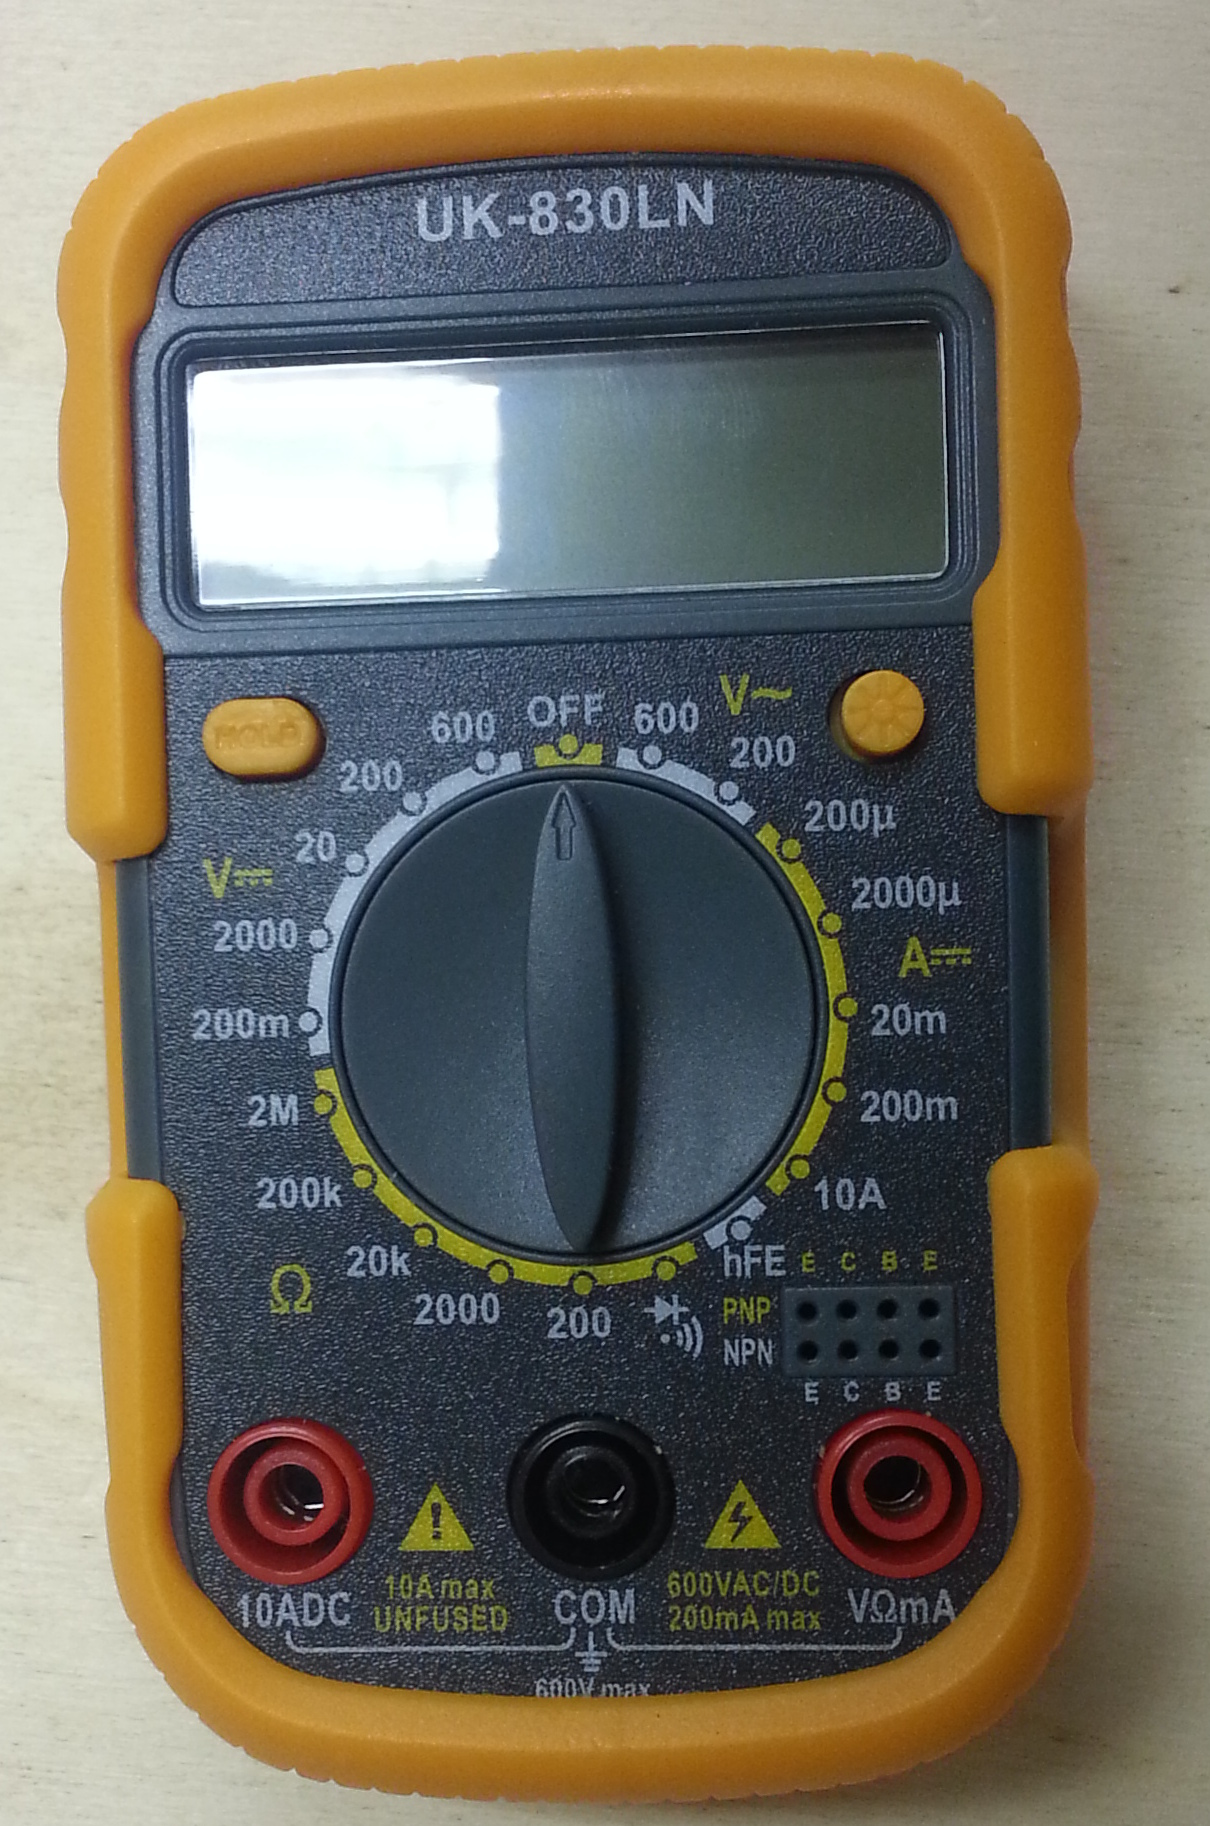
\includegraphics[width= 5cm]{./img/M_small.jpg}
				\label{fig:figure3}
			\end{figure}

			per ora non ci preoccupiamo troppo di come si collega, ve lo diciamo noi, ma appena avremmo imparato ad usare bene la legge di ohm capiremmo tutto		
		\end{frame}

		\begin{frame}[c]\frametitle{I nostri multimetri}
		    
			\begin{figure}[tb]
				\centering
				\includegraphics[width= 5cm]{./img/M_big.jpg}
				\label{fig:figure3}
			\end{figure}

			per ora non ci preoccupiamo troppo di come si collega, ve lo diciamo noi, ma appena avremmo imparato ad usare bene la legge di ohm capiremmo tutto		
		\end{frame}
	% section il_multimetro (end)

	\section{Il nostro primo circuito} % (fold)
	\label{sec:il_nostro_primo_circuito}

		\begin{frame}[c]\frametitle{Il nostro primo circuito}
			\centering
			\begin{circuitikz} 
				\draw (0,0)
      			to[battery,v=$V_0$] (0,2) % The voltage source
     			to[short] (2,2)
      			to[R=$R$] (2,0) % The resistor
     			to[short] (0,0);
			\end{circuitikz}
		\end{frame}

		\begin{frame}[c]\frametitle{Il nostro primo circuito}
		    \centering
			\begin{circuitikz} 
			\draw (0,0)
      			to[V,v=$V_0$] (0,2) % The voltage source
     			to[short] (2,2)
      			to[R=$R$] (2,0) % The resistor
     			to[short] (0,0);
			\end{circuitikz}
		
		
		\end{frame}

		\begin{frame}[c]\frametitle{Il nostro primo circuito}
		    \centering
			\begin{circuitikz} 
			\draw (0,0)
      			to[V,v=$V_0$] (0,2) % The voltage source
     			to[ammeter] (2,2)
      			to[R=$R$] (2,0) % The resistor
     			to[short] (0,0);
     		\draw (2,2)
     			to [short] (4,2)
     			to [voltmeter] (4,0)
     			to [short] (2,0);
			\end{circuitikz}		
		\end{frame}	
	% section il_nostro_primo_circuito (end)

%%% Local Variables:
%%% mode: latex
%%% TeX-master: "slide"
%%% End:
